%%%%%%%%%%%%%%%%%%%%%%%%%%%%%%%%%%%
%This is the LaTeX ARTICLE template for RSC journals
%Copyright The Royal Society of Chemistry 2016
%%%%%%%%%%%%%%%%%%%%%%%%%%%%%%%%%%%

\documentclass[3p,preprint,review]{elsarticle}

\usepackage[version=3]{mhchem}
%\usepackage[left=1.5cm, right=1.5cm, top=1.785cm, bottom=2.0cm]{geometry}
\usepackage{balance}
\usepackage{mathptmx}
\usepackage{sectsty}
\usepackage{graphicx}
\usepackage{subcaption}
\usepackage{lastpage}
%\usepackage[format=plain,justification=justified,singlelinecheck=false,font={stretch=1.125,small,sf},labelfont=bf,labelsep=space]{caption}
\usepackage{float}
\usepackage{fancyhdr}
\usepackage{fnpos}
\usepackage{enumitem}
\usepackage[english]{babel}
\addto{\captionsenglish}{%
	\renewcommand{\refname}{Notes and references}
}
\usepackage{array}
\usepackage{droidsans}
\usepackage{charter}
\usepackage[T1]{fontenc}
\usepackage[usenames,dvipsnames]{xcolor}
\usepackage{setspace}
\usepackage[compact]{titlesec}
\usepackage{hyperref}
\usepackage{todonotes}
\usepackage{siunitx}
%Figuras al final
\usepackage[nomarkers,figuresonly]{endfloat}

\graphicspath{{Figures/}}
\biboptions{super,sort&compress,comma}

\title{Characterization of an anionic membrane mimetic with natural phospholipid
	contend and magnetic
	orienting capabilities}

\author[1]{D. Muñoz-Gacitúa\corref{cor1}}
\author[2]{Matias Monroy-Cárdenas}
\author[2]{R. Araya-Maturana}
\author[1]{B. Weiss-López}

\cortext[cor1]{E-mail address:\texttt{diego.munoz.g@ug.uchile.cl}}

\address[1]{Laboratorio de Fisicoquímica Molecular, Facultad de Ciencias,
	Universidad de Chile, Santiago, Chile}
\address[2]{Instituto de Química de Recursos Naturales, Universidad de Talca,
	Talca, Chile.}

\begin{document}
	
	\begin{abstract}
		The cellular membrane is a highly complex and dynamical structure, with
		variable and inhomogeneous composition, which makes detailed structural studies
		a very difficult task. $^2$H-NMR has become one of the most useful tools for
		many of such studies, however this requires the use of simpler structures that
		behave as close as possible to the cellular membrane, i.e. membrane mimetics. In
		this article we present a new anionic nematic lyotropic liquid crystal, with an
		important content of a natural mixture of phospholipids isolated from soybean,
		which can be employed as membrane mimetic. The capability of the mesophase to
		spontaneously orient when exposed to an external magnetic field, enables it for
		studies about distribution, dynamics and mobility of mesophase components, as
		well as dissolved substrates, employing $^2$H-NMR. A $^2$H-NMR characterization
		of the mimetic is performed by using different deuterated probes. To validate
		its permeability properties as membrane, the permeating capability of Benzocaine
		and the inability of Levodopa to do so were tested. For an atomic detailed
		characterization of both, the new mimetic and the process of crossing the
		interface, we also present a molecular dynamics simulation calibrated to
		reproduce experimental $^2$H-NMR results.
	\end{abstract}
	
	\begin{keyword}
		Membrane mimetic \sep $^2$H-RMN \sep Molecular dynamics
	\end{keyword}
	
	\maketitle
	
	\renewcommand{\thefootnote}{\alph{footnote}}
	\section{Introduction}
	The cell is a highly complex unit present in all living organisms: it
	constitutes the building block of life. Essentially, consists in a closed
	domain
	containing smaller organelles in a highly complex and crowded aqueous solution,
	all enclosed by a bilayer made of mainly phospholipids and containing fatty
	acids, sugars, cholesterol and proteins, among others. This bilayer is called
	cell membrane or cytoplasmic membrane. Membranes itself are very complex
	molecular organizations with variable and inhomogeneous composition, and its
	atomic level understanding is a very difficult task. For this reason, the
	employment of
	membrane mimetics and models has become common practice.\cite{Bondar2019}\\
	Because of their ability to orient spontaneously when exposed to an external
	magnetic field, bilayered micelles, also called ``bicelles'', have been widely
	used as membrane mimetics, as they allow the use of solution NMR to probe the
	orientation and dynamics of liposomes and
	drugs\cite{Beaugrand2016,Montecinos2007,Ruiz-Fernandez2016}. Although a
	composition capable of forming magnetic orienting bicelles was described in the
	late 1960s\cite{Lawson1967}, the authors did not recognize the bicelle structure
	at the time, instead, ten years later Amaral \textit{et al.} were the first to
	identify the bicelle structure
	with a mixture of sodium decyl sulphate and
	1-decanol\cite{Amaral1979}. Later,
	in the 1990s, it was discovered that a
	mixture of DMPC\footnote{1,2-dimyristoyl-\textit{sn}-glycero-3-phosphocholine}
	and
	CHAPSO\footnote{3-(cholamidopropyl)dymethylammonio-2-hydroxy-1-propanesulfonate}
	forms magnetically orientable bicelles\cite{Sanders1990}, these aggregates are
	suitable to use as a membrane mimetics, as they contain
	phospholipid in their composition. Many improvements have been made to this
	composition over the years. It was found that CHAPSO can be replaced by
	DHPC\footnote{1,2-dihexanoyl-\textit{sn}-glycero-3-phosphocholine} which has a
	structure that resembles more to a natural phospholipid\cite{Sanders1992}, it
	was also found
	that the addition of cholesterol improves the stability of the
	bilayer\cite{Shapiro2010} and
	the addition of Triton X-100 detergent improves its magnetic orienting
	capabilities\cite{Park2010}. Nowadays, bicelles are considered good membrane
	mimetics, as they have been successfully employed to predict drug permeability
	through the membrane\cite{Sun2008,Durr2013,Matsumori2007,Koenig2005}, and to
	elucidate
	protein structures in the trans-membrane domain\cite{Durr2012}. The use of
	bicelles is ideal when
	the
	drug-detergent (or protein-detergent) complex is small (<\SI{100}{kDa}), as
	these systems can be studied in solution
	NMR\cite{Warschawski2011,Raschle2010,Sanders2006}. However, it should be
	pointed out that a single phospholipid bilayer by no means represents the
	complexity of the mixture found in natural membranes.\\
	
	Membrane proteins play a significant role in human
	pathologies\cite{Birnbaumer1999,Gillet2010}. About 30\% of human genes code for
	membrane proteins\cite{Fagerberg2010} and they are targeted by more than 50\%
	of
	drugs\cite{Warr1986,Wallin2008}. Therefore, most drugs have to cross membrane
	interfaces to reach their active site, and consequently, the activity of these
	drugs depends, among other factors, on their ability to perform this task. For
	this reason, it is important for a membrane mimetic to be able to reproduce
	permeation of drugs and proteins, as they would on a cellular membrane. As a
	way
	of testing permeability properties of the membrane mimetic developed in this
	article, we employ Benzocaine
	and Levodopa, whose penetrating activity (or lack of) has been studied in
	detail before.\\
	% This is particularly true for local anesthetics (LA). For more than hundred
	% years it has been observed that the effectiveness of many LA correlates
	% positively with
	% lipophilicity\cite{Meyer1899,Overton1901,Langerman1994a,Langerman1994},
	%showing
	% the importance of becoming incorporated into the bilayer. It is widely
	%accepted
	% that inhibition of voltage gated \ce{Na+} channels is directly involved in
	%the
	% mechanism of LA\cite{Hille1977,Wang1998} and three possible pictures have
	%been
	% proposed: (a) LA directly binds the pore of the channel blocking the transit
	%of
	% ions, (b) LA reaches the active site by one of the lateral cavities filled
	%with
	% hydrophobic membrane components, and (c) the presence of LA near the
	%interface
	% modifies the structure and dynamics of the bilayer itself, perturbing the
	% conformational dynamics and functioning of the
	%
	
	
	
	
	%channel\cite{Oakes2019,Martin2014,Shibata2005,Griepernau2007,EmmaTerama2008,DePaula2008,Cantor1998,Bernardi2009,Godwin2005}.
	% Despite which mechanisms are actually taking place, crossing membrane
	%interfaces
	% to become incorporated into the hydrophobic domain appears to be a crucial
	%step
	% for
	% most drugs.\\
	Benzocaine is a well-known local anesthetic for topical use. It has been widely
	employed anesthetizing the oropharynx for trans-esophageal echocardiography,
	bonchoscopy, esophagogastroduodenoscopy, in cold sores, mouth ulcers,
	toothache,
	sore gums and denture ache among others\cite{McEvoy2007}.
	% A significant number of
	% cases of Benzocaine induced cyanosis (methemoglobinemia) have been reported
	% along the
	% years\cite{Lardieri2019}, however it still remains in use.\\
	Benzocaine has been subject of a significant number of studies, including free
	energy transfer from water to the interior of different membrane
	mimetics\cite{Martin2014a,Cascales2011,Porasso2009,J.J.LopezCascales2006},
	estimations about location and orientation in different bilayers and
	monolayers\cite{Matsuki2001,Suwalsky2004,Kuroda2000,Choi2001}, interactions
	with
	a variety of
	solvents\cite{Cardenas2016,Cardenas2018,Paluch2015,Avila2002,Aguado2013} and
	encapsulation in different structures for controlled delivery
	purposes\cite{Shkurenko2018,AttouiYahia2017,Li2016,Arantes2014,Puglia2011}
	among
	others. All the evidence confirms that Benzocaine is able to cross the
	interface
	of membrane mimetics to become incorporated into the
	hydrophobic bilayer to finally be located at the inner interface.\\
	Contrary to most local anesthetics, Levodopa (or L-DOPA), the precursor of the
	neurotransmitter dopamine, commonly used in treatment of Parkinson's
	disease\cite{Fabbrini1987},
	is
	able to cross membrane interfaces only via active
	processes\cite{BENTLEY2012349,PRYOR2013180}.
	Therefore, in the absence of appropriate specific receptors, Levodopa should
	remain attached to the outer interface and should not reach the hydrophobic
	bilayer core\cite{Orowski2012}.\\
	
	In this article, we present a new anionic nematic lyotropic liquid crystal,
	with bilayer structure, susceptible to be used as membrane mimetic. It is made
	of sodium dodecyl sulfate (SDS), 1-decanol (DeOH), sodium sulphate
	(\ce{Na2SO4})
	and a mixture of natural phospholipids extracted from soybean, all dissolved in
	water. The structure of the mesophase, which spontaneously orients in magnetic
	fields,
	was characterized using polarized light microscopy textures and to observe the
	dynamics
	of the interface as well as deeper into the hydrophobic core, $^2$H-NMR
	quadrupole splittings from HDO, DeOH-$\alpha$-d$_2$, and SDS-d$_{25}$ were
	measured. To test the capability of the new mimetic to reproduce
	cell membrane behavior, Benzocaine and Levodopa were dissolved in the mesophase
	solution. According to previous evidence, Benzocaine should spontaneously be
	incorporated inside the bilayer and become located around the inner
	interface\cite{Martin2014a},
	whereas Levodopa should remain attached to the outer
	interface\cite{Orowski2012}. 
	To obtain an atomic detailed characterization of the mimetic dynamics and
	structure, including information about location, interface crossing dynamics
	and
	interactions of Benzocaine and Levodopa with the bilayer components, the
	spectroscopic measurements were complemented with classical molecular dynamics
	(MD) simulations.
	
	\section{Materials and methods}
	\subsection{Materials.}
	The reagents SDS, SDS-d$_{25}$, sodium sulphate and a phospholipid mixture
	extracted from soybean were purchased from \textit{Sigma Aldrich}. DeOH,
	deuterium oxide and HPLC-grade water were purchased from \textit{Merck}. All
	these reagents were employed without alterations, excepting sodium sulphate
	which was oven dried 24 hours before used. Deuterated 1-decanol
	(DeOH-$\alpha$-d$_2$) was synthesized by reducing ethyl decanoate
	(\ce{C12H24O2}) with lithium aluminum deuteride (\ce{LiAlD4}) and
	purified by vacuum fractional distillation.\\
	\subsection{Sample preparation.}
	Samples were prepared by mixing each dry component (SDS, \ce{Na2SO4} and
	phospholipid mixture) in a \SI{5}{mL} centrifuge tube, and then adding DeOH and
	deuterium enriched water(\SI{0.5}{\percent}$\tfrac{v}{v}$\ce{D2O}), with each
	component
	weighted and added in proportion according to Bahamonde's
	bicelle\cite{Bahamonde-Padilla2013}. Phospholipid content was added while
	keeping the rest of the components in
	proportion. Each sample is then submitted to a
	rotational mixer at \SI{4}{rpm} for 24 hours at a temperature of
	\SI{37}{\celsius}, and then centrifuged at \SI{6000}{rpm} for 3 minutes.
	
	
	\subsection{Nuclear magnetic resonance}
	\label{sec:method_nmr}
	All solution $^2$H-NMR experiments were carried out on a Bruker Avance 400
	spectrometer (Universidad de Santiago de Chile, Santiago, Chile) operating at
	\SI{61.422}{MHz}. Spectra were obtained with a $\pi/2$ pulse length of
	\SI{22.4}{\micro\second}, an acquisition time of \SI{760}{ms}, an spectral
	width of \SI{43.1}{kHz} in \SI{32}{kb} files with a digital resolution of
	\SI{1.32}{Hz} per point.
	256 scans were acquired per spectrum. Spectra
	were acquired at \SI{37}{\celsius}, and a 10 minute pre-acquisition delay was
	employed to allow each sample to reach thermal equilibrium. Spectra were
	processed
	using Bruker TopSpin 4.0 software.
	
	\subsection{Molecular dynamics}
	
	MD calculations were performed in the National Laboratory for High Performace
	Computing (Universidad de Chile, Santiago, Chile).
	All simulations were performed using the GROMACS-2016\cite{Abraham2015}
	software
	bundle. A cutoff scheme was used for non-bonding interactions according to each
	force-field recommendation values, and long range electrostatic interactions
	were calculated employing the particle mesh Ewald method\cite{DiPierro2015}.
	Temperature control was achieved with a modified Berendsen
	thermostat\cite{Bussi2007} with a time constant of \SI{1.0}{ps}, while pressure
	was equilibrated with a semi-isotropic Berendsen barostat\cite{Berendsen1984}
	with a time constant of \SI{1.0}{ps} for both xy-plane and z-axis. Both,
	temperature and pressure were adjusted to \SI{310}{K} and \SI{1}{bar}
	respectively. Periodic
	boundary conditions were applied on all three dimensions.\\ Several force
	fields were tested.
	Before each production simulation, a short equilibration run was performed for
	a
	duration of \SI{1}{ns} with an integration time-step of \SI{1}{fs}. Afterwards,
	each production run was calculated to a duration of \SI{40}{ns} with an
	integration time-step of \SI{2}{fs}. TIP3P water
	model\cite{Neria1996,Jorgensen1983} was employed on the
	simulation with CHARMM36 force-field, while SPC/E\cite{Berendsen1987} was
	employed on simulations
	with Berger and Gromos53A6 force-fields. The same initial configuration was
	employed to test each force-field, and it was generated using software
	Packmol\cite{Martinez2009} arranging a bilayer with composition in the same
	proportion as the membrane mimetic in table \ref{tab:mimetic_composition} to a
	total of 9613 molecules. The phospholipid mixture was simulated as a mixture of
	39\%
	PLPC\footnote{1-palmitoyl-2-linoleoyl-\textit{sn}-glycero-3-phosphocholine},
	26\% DLPC\footnote{1,2-dilinoleoyl-\textit{sn}-glycero-3-phosphocholine}, 24\%
	DLPE\footnote{1,2-dilinoleoyl-\textit{sn}-glycero-3-phosphoethanolamine} and
	11\% DOPE\footnote{1,2-dioleoyl-\text{sn}-glycero-3-phosphoethanolamine}. These
	proportions were chosen in accordance with the composition of the phospholipid
	mixture employed, as
	reported by the vendor.\\
	PMF calculations were performed employing the Umbrella Sampling/WHAM
	method\cite{Kumar1992}. The starting configuration of each simulation window
	employed for the PMF calculation was generated from a trajectory of the target
	molecule pulling away from the center of the bilayer, making a starting point
	each \SI{1.5}{\angstrom}, up to \SI{4.5}{nm} making a total of 30 simulation
	windows. Each simulation window was calculated with the same parameters as the
	calibrated model shown ahead, up to a total of \SI{20}{ns} on each window, with
	a weak harmonic force with constant
	\SI{240}{\kilo\joule\per\mole\per\nano\meter\squared} applied on the bilayer
	in order to maintain its shape and position during the course of each
	simulation window.\\
	
	\section{Results and discussion}
	
	\subsection{Preparation of the membrane mimetic}
	
	\begin{figure}[h]
		\centering
		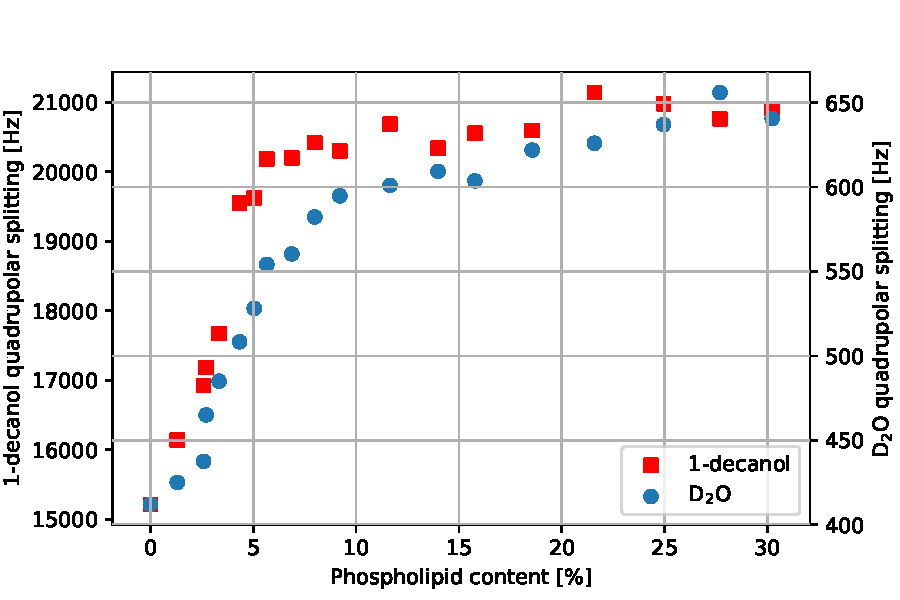
\includegraphics[width=\columnwidth]{splitting_v_phospholipid}
		\caption{Quadrupolar splittings of 1-decanol-$\alpha$-$d_2$ and \ce{D2O} in
			$^2$H-RMN as a function of the phospholipid content in the mimetic.}
		\label{fig:1st_max}
	\end{figure}
	
	In order to achieve a membrane mimetic that behaves as similar as possible to
	the actual cellular membrane, it is necessary to maximize its phospholipid
	concentration. This is important considering that multiple researchers have
	concluded that there are specific interactions between phosphate from the
	multiple phospholipids and certain amino-acids that modify the membrane
	permeability where this interaction occurs\cite{Aliaga2011,Hristova2011}.\\
	Also, the membrane mimetic must orient itself in presence of an external
	magnetic field. This is so the deuterated probes in the mimetic can produce a
	\textit{quadrupole splitting} in a solution $^2$H-RMN spectrum, which will be
	used to calibrate the MD simulations. This calibrated simulation can be used to
	assess other properties, not possible to measure experimentally, with more
	confidence.\\
	
	Both these requirements were fulfilled by employing the membrane mimetic
	studied by Bahamonde \textit{et al}\cite{Bahamonde-Padilla2013} as starting
	point, then introducing and maximizing the concentration of phospholipid. The
	maximization was performed in two steps. In a first step,
	a batch of membrane mimetic was prepared, each one with an increasing amount
	of
	phospholipid from 0\% up to 30\%$\tfrac{w}{w}$  (see figure \ref{fig:1st_max}),
	$^2$H-RMN
	spectra from HDO and DeOH-$\alpha$-$d_2$; and polarized light microscopy
	pictures were taken to each prepared
	membrane mimetic. From these, the composition with 22\%$\tfrac{w}{w}$ of
	phospholipid was
	chosen to continue with the next maximization step, as this was the composition
	with highest phospholipid content that retained a $^2$H-NMR spectrum
	characteristic of a bilayered nematic phase.\\
	\begin{figure}[h]
		\centering
		\begin{subfigure}{0.45\columnwidth}
			\includegraphics[width=\linewidth]{schlieren_1max}
			\caption{4\% Phospholipid}
			\label{fig:schlieren}
		\end{subfigure}
		\begin{subfigure}{0.45\columnwidth}
			\includegraphics[width=\linewidth]{oily_17percent}
			\caption{17\% Phospholipid}
			\label{fig:oily}
		\end{subfigure}
		\caption{Polarized light microscopy pictures of membrane mimetics at different
			phospholipid concentration. Both pictures taken at 100x magnification.}
		\label{fig:plm}
	\end{figure}
	During this step of maximization, we noticed a phase transition upon reaching
	8\%$\tfrac{w}{w}$ of phospholipid content, this phase transition was also
	evidenced by
	polarized light microscopy (see figure \ref{fig:plm}) where a transition from a
	\textit{Schlieren} pattern (fig. \ref{fig:schlieren}) to an \textit{oily
		streak}
	pattern (fig. \ref{fig:oily}) was observed. A similar transition has been
	observed before while studying cationic lipid based
	bicelles\cite{ruiz2016effect},
	the transition was attributed to a change from a monoaxial disc-shaped bicelles
	to a biaxial elongated bicelles. We believe a similar phase transition occurs
	in our
	case, considering that the oriented bilayer structure remains, as evidenced by
	the $^2$H-NMR quadrupolar splittings.\\
	
	A second maximization step was performed by reducing the amount of SDS used to
	prepare each mimetic and subsequently adding phospholipid until a nematic phase
	was no longer obtained. The results from the membrane mimetic candidates
	prepared in this step are summarized in figure \ref{fig:phase_diag}. From these
	preparations, the composition with the highest phospholipid content that
	retained a nematic phase was chosen for further experimentation. The exact
	composition of the membrane mimetic is detailed in table
	\ref{tab:mimetic_composition}
	
	\begin{figure}[h]
		\centering
		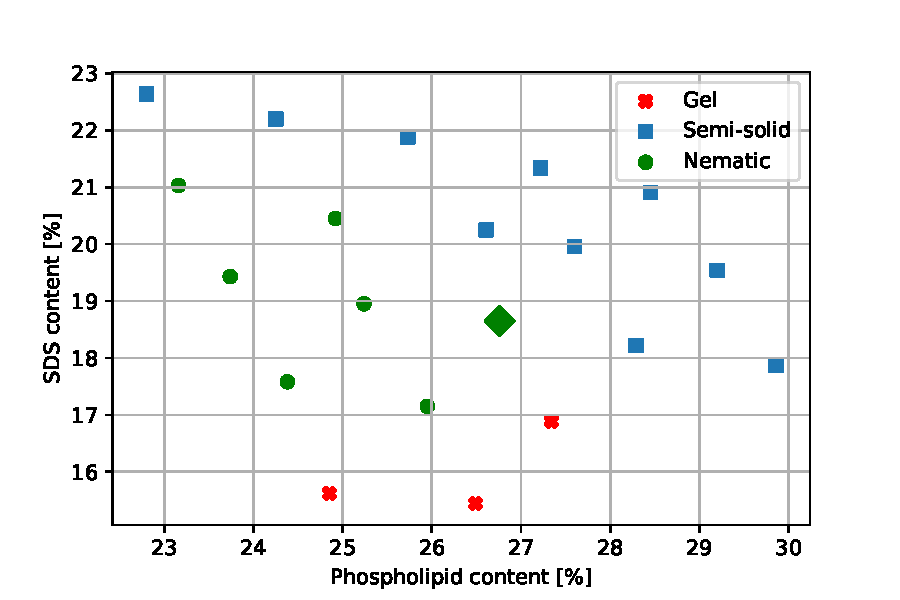
\includegraphics[width=\columnwidth]{phase_diag}
		\caption{Partial phase diagram of the membrane mimetic when varying SDS and
			phospholipid content. The selected composition is marked as a green
			diamond.}
		\label{fig:phase_diag}
	\end{figure}
	
	\begin{table}[h]
		\small
		\caption{\ }
		\label{tab:mimetic_composition}
		\begin{tabular*}{0.96\columnwidth}{@{\extracolsep{\fill}}ll}
			\hline
			Compound & Content [$\%\tfrac{w}{w}$] \\
			\hline
			Sodium dodecyl sulphate &  18.65\% \\
			Sodium sulphate & 1.55\%  \\
			1-decanol & 3.92\%  \\
			Phospholipid mixture & 26.76\%  \\
			Water & 49.12\% \\
			\hline
		\end{tabular*}
	\end{table}
	
	\subsection{$^2$H-NMR and calibration of a computational model}
	\label{sec:calib}
	
	In order to obtain more reliable information from a molecular dynamic
	simulation,
	it is desirable that experimentally measured properties are well reproduced by
	calculations. That said, MD has to be calibrated to reproduce known experimental
	results, which is why
	we
	tested multiple force-fields to see which one yields a closer representation of
	the aliphatic chain dynamics, evidenced by reproducing $^2$H-RMN quadrupole
	splittings. Figure \ref{fig:reference} shows the $^2$H-NMR spectrum of the
	membrane mimetic prepared according to the composition stated in table
	\ref{tab:mimetic_composition}, enriched with \ce{H2O}(0.5\% of the total
	\ce{H2O} replaced by \ce{D2O}) and SDS-d$_{25}$(10\% of the total SDS replaced
	by SDS-d$_{25}$). The quadrupolar splitting of each C-D bond depends largely on
	their order parameter ($S_{CD}$, see equation \ref{eq:splitting}), therefore it
	makes sense to assign each quadrupolar splitting from the least ordered to the
	most ordered methylene, resulting as follows: The central signal arises from an
	average in time of HDO oriented at the interface in fast exchange with
	non-oriented HDO at the bulk (smallest splitting, \SI{388}{Hz}. Not shown). The
	next less split signal arises from the deuterated methyl group (\ce{CD3}-)
	capping the tail of each SDS-d$_{25}$, as the rotation of this group produces a
	lower order parameter, the smallest along the chain. The rest of the more split
	signals correspond to subsequent deuretated methylenes (-\ce{CD2}-), with the
	ones closer to the charged sulphate head-group having a higher quadrupolar
	splitting, since the strong Coulombic interaction between this charged end and
	the interface produces a restraining effect on the movement of the nearby
	deuterons. The adjustment of the simulation relies on the accurate reproduction
	of these quadrupolar splittings from SDS-d$_{25}$, as they reflect the dynamics
	of the lipid chains in the bilayer.\par
	\begin{figure}[h]
		\centering
		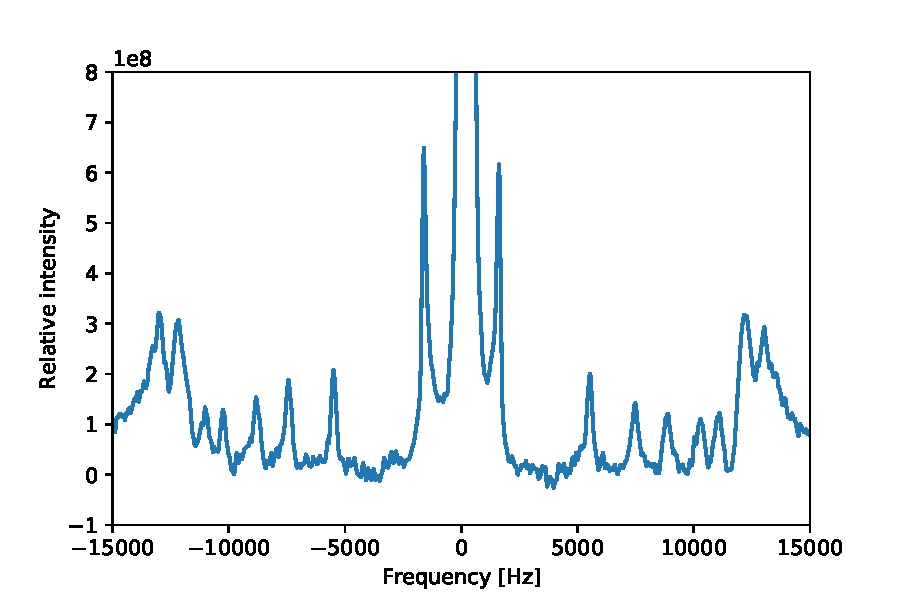
\includegraphics[width=\columnwidth]{nmr_reference}
		\caption{$^2$H-NMR spectrum of membrane mimetic enriched with SDS-d$_{25}$.
			Central peak (not shown completely) belongs to \ce{HDO} present in the
			sample, while the rest of the signals are split SDS-d$_{25}$ signals which
			were used as reference to calibrate a computational model.}
		\label{fig:reference}
	\end{figure}
	Initially,
	three force-fields with different partial charge distributions were tested.
	These force-fields were chosen due to their ability to reproduce other
	structures of
	SDS aggregates\cite{Tang2014}.\par
	The tested force-fields were:
	\begin{itemize}
		\item CHARMM36\cite{Vanommeslaeghe2009}
		\item Berger\cite{Berger1997} with partial charge distribution according to
		Merz-Kollman
		method\cite{Besler1990}
		\item Berger with partial charge distribution according to
		Gromos53A6\cite{Oostenbrink2004}
		parameters.
		\item Gromos53A6 with partial charge distribution according to Merz-Kollman
		method.
		\item Gromos53A6 with partial charge distribution according to its own
		parameters.
	\end{itemize}
	
	From each resulting simulation run, deuterium order parameters ($S_{CD}$) were
	calculated for the SDS aliphatic chain, which were used to calculate a
	predicted
	quadrupolar splitting employing equation (\ref{eq:splitting}). These order parameters, in turn, depend on the angle ($\phi$) between the corresponding carbon-deuterium bond vector and the bilayer normal (see equation \ref{eq:order}). The angular brackets represent molecular and temporal ensemble averages.
	\begin{equation}
	\label{eq:order}
	S_{CD} = <3 \cos^2\phi -1>/2
	\end{equation}
	\begin{equation}
	\label{eq:splitting}
	\Delta\nu = \frac{3}{4} \frac{e^2qQ}{h}(3\cos^2\theta - 1) S_{CD}
	\end{equation}
	These
	quadrupolar splittings also depend on
	a
	coupling constant ($e^2qQ/h$, \SI{170}{kHz} for aliphatic
	deuterons\cite{Davis1983}) and the angle ($\theta$) between the normal to the
	bilayer and the
	applied magnetic field. Software \texttt{gmx order}, included in GROMACS, was
	employed to calculate the deuterium order parameter from each simulation.
	

	
	The calculated quadrupolar splittings were compared with the experimental
	$^2$H-NMR values and are
	displayed in figure \ref{fig:calibration}. It is observed that employing
	Gromos53A6 force-field yields results that are closer to experimental ones,
	obtaining a good correlation for the carbons
	near the interface but with a small discrepancy towards the interior of the
	bilayer. This means that, in the simulation, the deuterons on the SDS chain are
	displaying more
	restricted dynamics than inferred from the $^2$H-NMR spectrum.
	
	\begin{figure}[h]
		\centering
		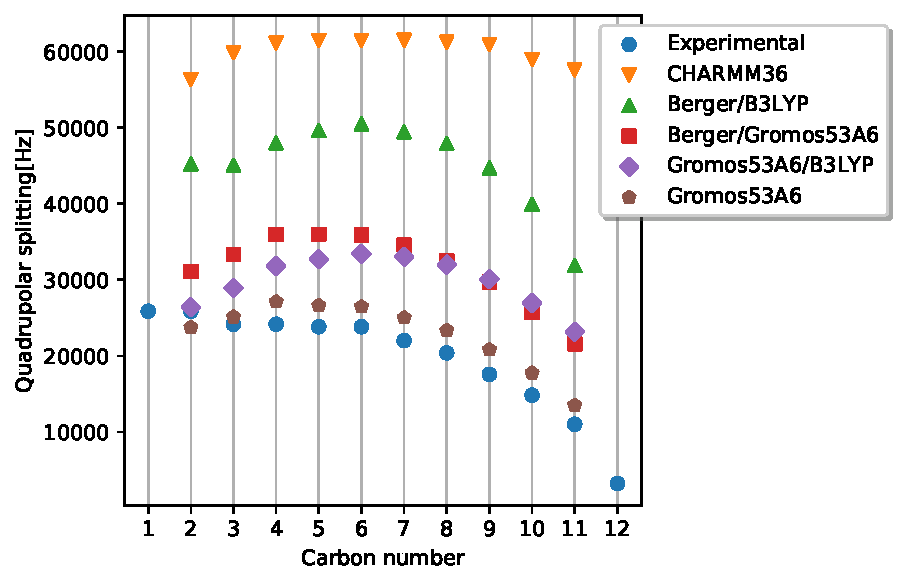
\includegraphics[width=\columnwidth]{calibration}
		\caption{Quadrupolar splittings of SDS-d$_{25}$ from a $^2$H-NMR. Comparison
			between experimental results and predicted by molecular dynamics employing
			different force-fields}
		\label{fig:calibration}
	\end{figure}
	
	Further improvement to the fitting of predicted splittings was done by
	employing
	two thermostats in the simulation, one governing the bulk solution with a
	reference temperature of \SI{310}{K} and another governing the bilayer
	components with a reference temperature of \SI{320}{K}, a little higher to
	introduce more kinetic energy to the chains. The reasoning behind
	this decision was based on the expectation that increased velocity on the
	bilayer components would have a greater effect on the mobility towards the
	center on the bilayer rather than in the interface, where Coulombic
	interactions
	are stronger and have a restraining effect on the mobility of the bilayer.
	After
	this adjustment, the simulation results in predicted quadrupolar splittings in
	very good agreement with the experimental ones, as shown in figure
	\ref{fig:2nd_calibration}.
	
	\begin{figure}[h]
		\centering
		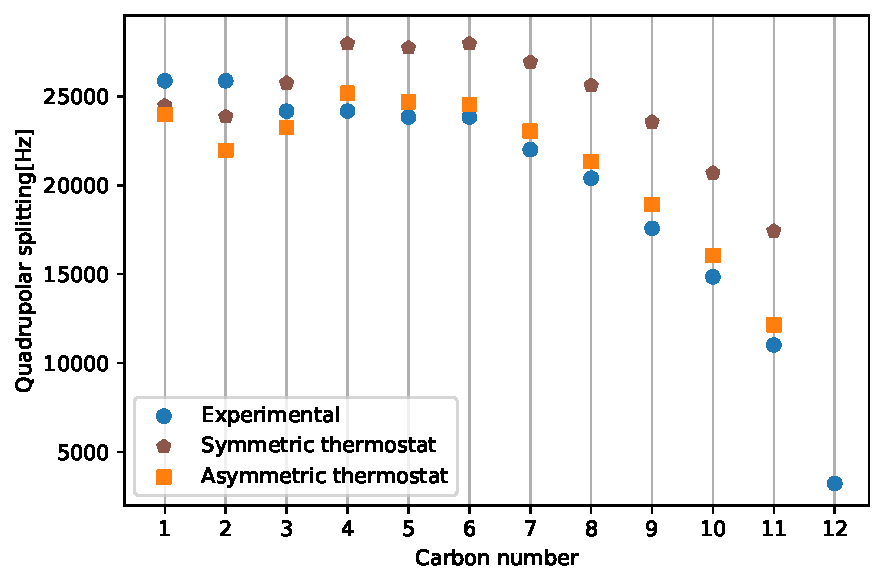
\includegraphics[width=\columnwidth]{calibration2}
		\caption{Quadrupolar splittings of SDS-d$_{25}$ from a $^2$H-NMR. Comparison
			between experimental results and predicted by molecular dynamics with
			symmetric and asymmetric thermostat}
		\label{fig:2nd_calibration}
	\end{figure}
	
	\subsection{Membrane mimetic characterization}
	\label{sec:characterization}
	
	Polarized light microscopy of the mesophase shows a thread-like pattern, this
	is
	characteristic of a lyotropic nematic phase\cite{dierking2006textures}.
	Furthermore, considering the magnitude of the measured quadrupolar
	splittings, and the fact that each methylene's deuteron pair in SDS-d$_{25}$
	yields
	a
	single quadrupolar splitting in solution $^2$H-NMR (see figure
	\ref{fig:reference}), we can conclude that this phase has a bilayer
	like structure with its bilayer normal perpendicular
	to the magnetic field ($\theta=\pi/2$ in eq. \ref{eq:splitting}). The
	posibility of a calamitic phase is discarded, since a calamitic phase implies a
	director axis being parallel to the magnetic field ($\theta=0$ in eq.
	\ref{eq:splitting}) which would produce splittings considerably smaller than
	observed.\\
	
	For a detailed characterization of the bilayer aggregate, a \SI{100}{ns}
	simulation run with the same settings as in the calibrated model was performed.
	To characterize the structure
	interface, charge density profiles were calculated for sodium, sulphate,
	dodecyl sulphate ions and phospholipids. (see figure \ref{fig:charge_density}).
	
	\begin{figure}[htb]
		\centering
		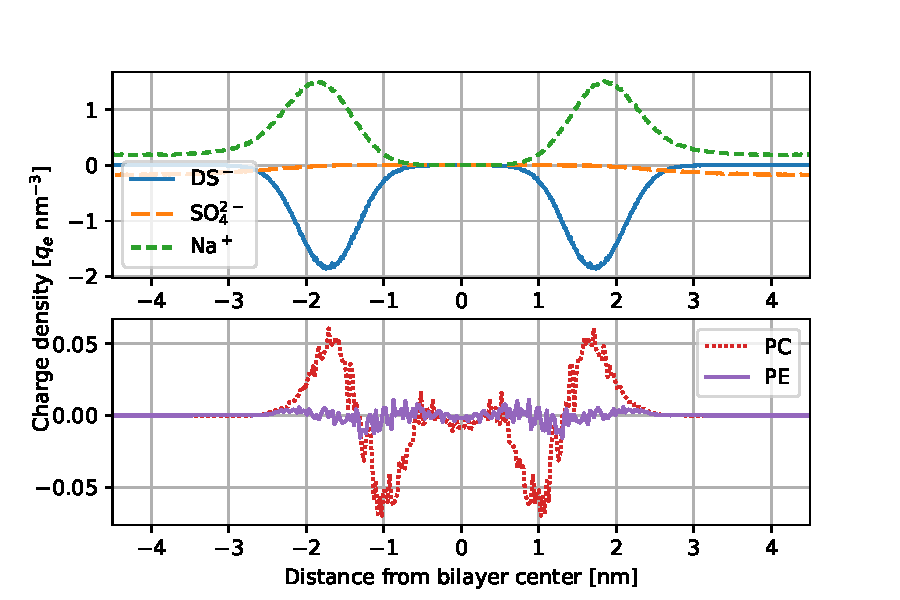
\includegraphics[width=\columnwidth]{charge_density}
		\caption{Charge density distribution of the simulated membrane mimetic. Dodecyl sulphate (\ce{DS-}) is shown as a continuous blue line, sulphate ions (\ce{SO4^{2-}}) as a orange long-dashed line, sodium ions (\ce{Na+}) as a green short-dashed line, phosphatidylcholines (PC) as a red dotted line and phosphatidylethanolamines as a continuous purple line.}
		\label{fig:charge_density}
	\end{figure}
	
	These charge density profiles show that phosphocholine's negatively charged
	phosphates reside inside the bilayer, around \SI{10.0}{\angstrom} from the
	center. With dodecyl sulphate's negative charge being stabilized partially by
	phosphocholine's quaternary ammonium, around \SI{17.4}{\angstrom} away from the
	bilayer center, and the counter-ion sodium peaking \SI{1.0}{\angstrom} further
	away at \SI{18.4}{\angstrom} from the bilayer
	center due to electrostatic attractions. The
	high charge polarization ($\sim\pm$\SI{1.5}{q_e \per\nano\cubic\meter}) present
	in
	this area acts as the main barrier against the crossing of polar compounds,
	such as
	zwitter-ionic Levodopa.\\
	
	A radial distribution function of water and sodium from sulfur in dodecyl
	sulfate yields a better picture on the role of water at the interface (see
	figure
	\ref{fig:rdf}). As can be seen from the radial distribution functions, a first
	layer of tightly oriented water molecules envelopes the outer layer of the
	membrane, with most of the sodium counter-ions locating further away from this
	water layer, at \SI{\sim 5}{\angstrom} from the sulfur. This makes sense if one
	considers that each sulfur in SDS is bonded by four oxygen atoms, three of
	which
	are pointing outwards the bilayer, so the closest atom to sulfur not only has
	to
	be positively charged, but also has to be small enough to fit between the
	oxygen
	atoms; for this reason is that water hydrogen is found closer to the bilayer
	center
	than sodium, despite the larger positive charge of the latter.
	\begin{figure}[htb]
		\centering
		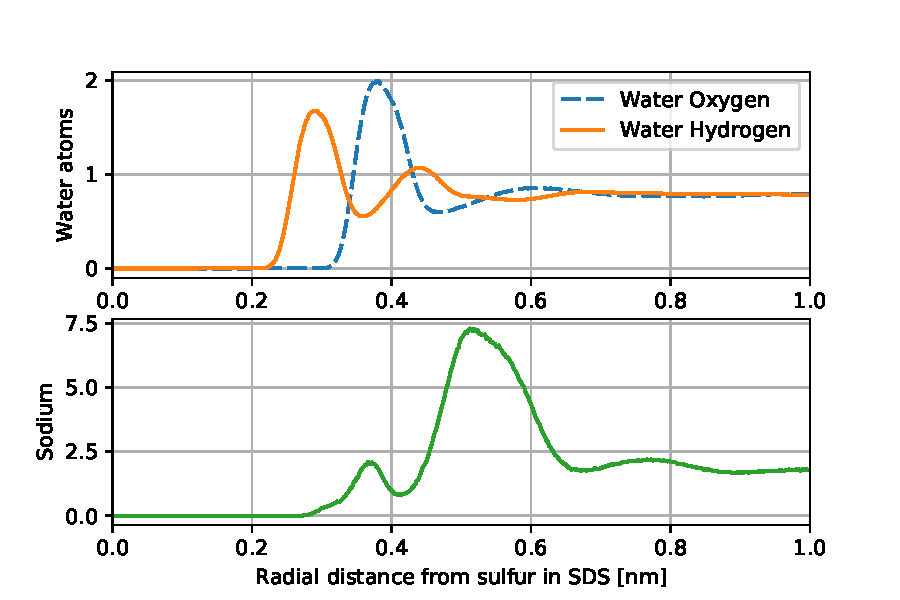
\includegraphics[width=\columnwidth]{rdf}
		\caption{Radial density function of water and sodium from sulfur in dodecyl
			sulphate.}
		\label{fig:rdf}
	\end{figure}
	
	\subsection{Membrane mimetic validation}
	\label{sec:validation}
	
	In order to corroborate that the prepared nematic lyotropic crystal behaves as
	a membrane mimetic, we tested the
	permeation properties of two well known drugs: Benzocaine, that is known to be
	able to
	passively
	cross the cellular membrane; and Levodopa, which is able to cross
	the
	cellular membrane only via active mechanisms, therefore it should not be able
	to
	permeate membrane mimetics without specific receptors.
	
	\subsubsection{Benzocaine control}
	\label{sec:benzo}
	
	A $^2$H-NMR spectrum from a membrane mimetic sample with \SI{8}{mg}
	Benzocaine added per gram of mimetic enriched with SDS-d$_{25}$ was obtained
	and compared
	with the spectrum of the same mimetic without the anesthetic (Differences
	displayed in figure
	\ref{fig:sds_benzocaine}). It can be seen that the presence
	of
	Benzocaine alters the quadrupolar splittings of the SDS aliphatic chain 
	from the first up to the sixth carbon, implying that Benzocaine is mostly
	residing in this zone, perturbing the order of these methylenes.
	\begin{figure}[htb]
		\centering
		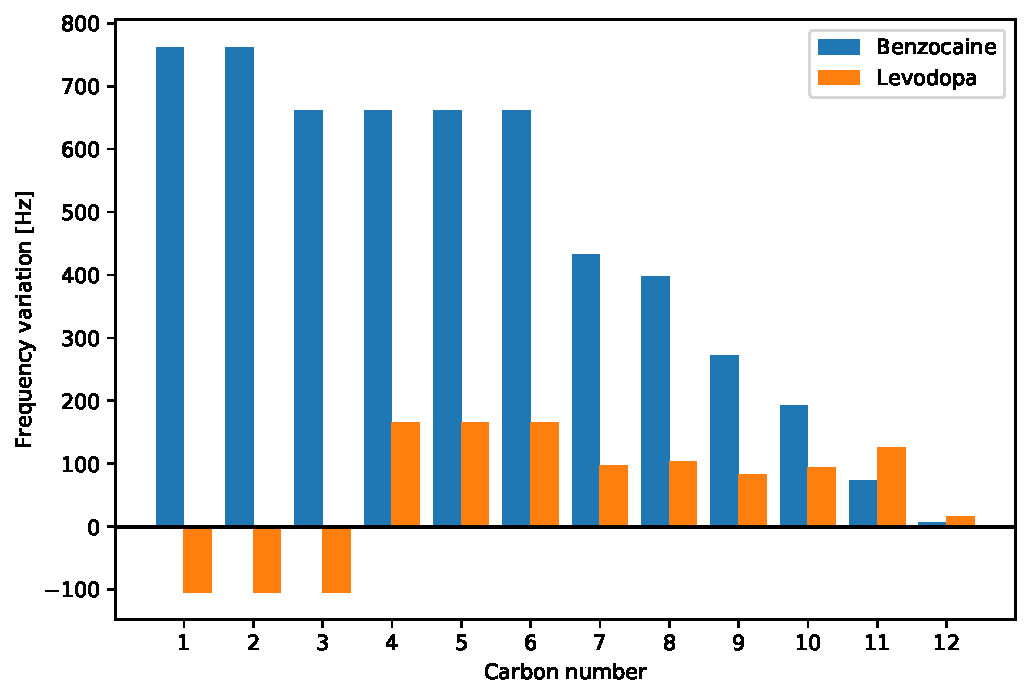
\includegraphics[width=\columnwidth]{sds_variation}
		\caption{Variation on quadrupolar splittings in $^2$H-NMR upon adding
			Benzocaine or Levodopa to a membrane mimetic sample enriched with
			SDS-d$_{25}$.}
		\label{fig:sds_benzocaine}
	\end{figure}
	Employing the calibrated model stated before, a potential of mean force (PMF)
	profile for the process of Benzocaine permeating the membrane mimetic along a
	path perpenticular to the interface, was calculated
	(figure \ref{fig:benzocaine_profile}). From this PMF profile it can be deduced
	that
	in order to complete its
	translocation, Benzocaine goes through three steps:
	First, it integrates spontaneously with the outer leaflet of the bilayer,
	without mayor interactions with the Stern layer, judged by the lack of an
	energy barrier in this area. Secondly, Benzocaine
	``flip-flops'' to the opposite leaflet of the bilayer with a small activation
	energy (\SI{11.2}{\kilo\joule}). And third and finally, it escapes the bilayer
	into the bulk at a minor energetic cost (\SI{27.1}{kJ}), showing that
	Benzocaine
	permeation through the membrane mimetic is indeed possible.\\
	\begin{figure}[htb]
		\centering
		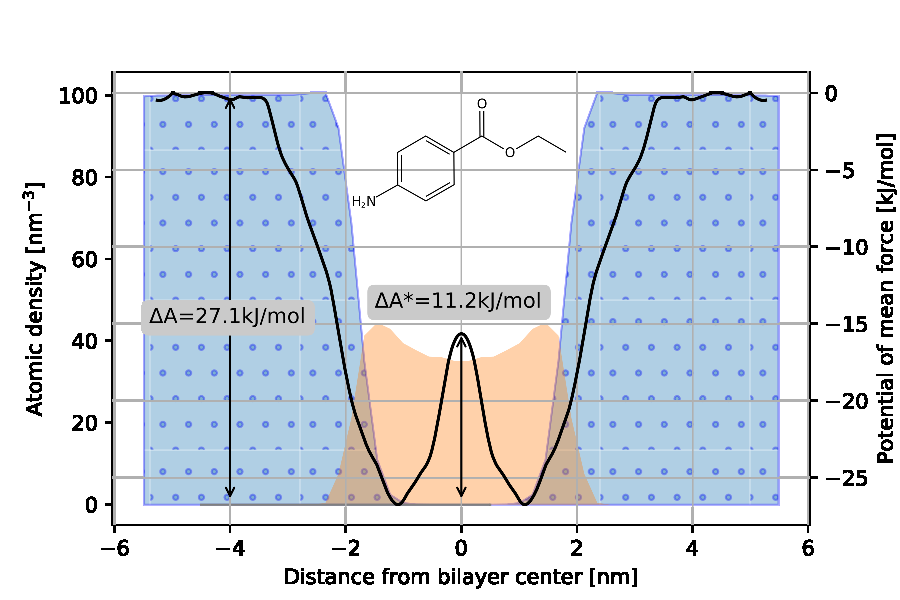
\includegraphics[width=\columnwidth]{benzo_profile_density}
		\caption{Mean force potential profile for the process of Benzocaine
			translocating through a membrane mimetic. The blue dotted area represents
			the water particle density, while the smooth orange area represents the
			lipid particle density in the simulation.}
		\label{fig:benzocaine_profile}
	\end{figure}
	This mechanism is in agreement with the spectroscopic results
	(displayed in figure \ref{fig:sds_benzocaine}), in both cases, the most
	probable
	position for Benzocaine to be in, is indeed inside the bilayer and close to the
	inner
	interface.\\
	
	\subsubsection{Levodopa control}
	\label{sec:ldopa}
	
	When studying the
	effects of adding \SI{7}{mg} of Levodopa per gram of membrane mimetic enriched
	with SDS-d$_{25}$, the effects are minor to negligible (see figure
	\ref{fig:sds_benzocaine}),
	implying that Levodopa is unable to enter the bilayer to alter
	the dynamics of the aliphatic chains.\\
	Employing the same method as in Benzocaine, a PMF profile was calculated for
	the
	process of Levodopa permeating the membrane mimetic (figure
	\ref{fig:levodopa_profile}). This profile shows that the lowest
	energy location for Levodopa to be in, is outside the bilayer, alongside the
	Stern
	layer.
	It also shows that in order to permeate the interface to translocate through
	the mimetic, Levodopa requires a rather
	large activation energy (\SI{102.4}{\kilo\joule\per\mol}), showing that a
	passive permeation of Levodopa mechanism is actually not possible at
	physiological temperature, as confirmed by $^2$H-NMR spectra. 
	\begin{figure}[htb]
		\centering
		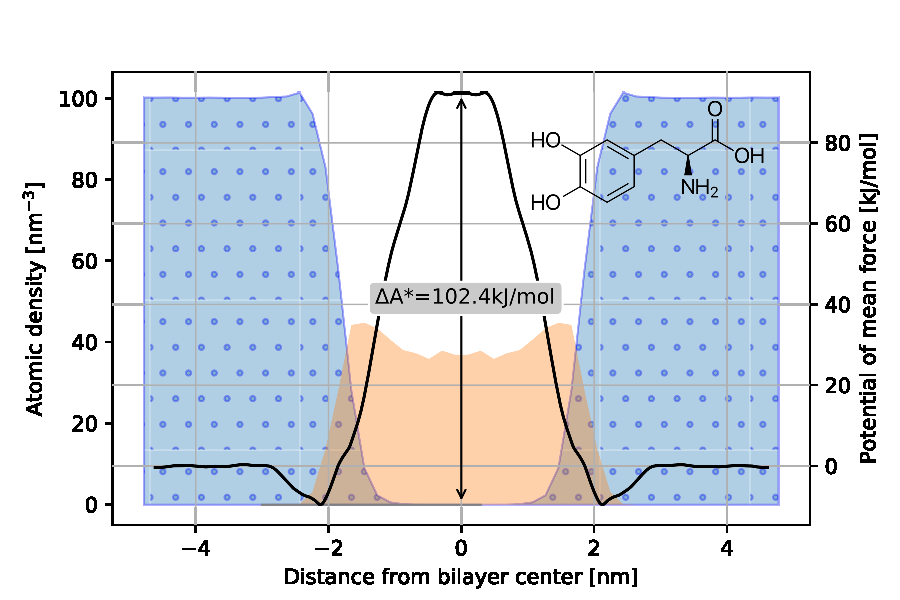
\includegraphics[width=\columnwidth]{ldopa_profile_density}    
		\caption{Mean force potential profile for the process of Levodopa
			translocating through a membrane mimetic. The blue dotted area represents
			the water particle density, while the smooth orange area represents the
			lipid particle density in the simulation.}
		\label{fig:levodopa_profile}
	\end{figure}
	
	
	
	\section{Conclusions}
	Multiple researchers\cite{Aliaga2011,Hristova2011} have found
	that there is a specific interaction between arginine and the phosphate group
	from
	phospholipids
	that modify the properties of the membrane where this interaction occurs.
	Therefore, the inclusion of an important amount of a natural phospholipid
	mixture makes this nematic lyotropic liquid crystal able to allow such
	interactions to occur, making this mimetic a closer representation of a real
	cellular membrane.\\
	Additionally, the low cost of this mimetic components, compared to the classic
	bicelles, makes it feasible to perform drugs and peptides permeability studies
	more massively.\\
	Also, the ability of the mesophase to orient itself in an external magnetic
	field
	makes this membrane mimetic useful for studies of structure and dynamics
	employing solution
	$^2$H-NMR.\\
	In addition, we have developed a MD model calibrated to reproduce
	experimentally measured mesophase order paramteres. Using this developed model,
	PMF profiles of Benzocaine and Levodopa crossing the bilayer interface were
	calculated, and the results reproduce the experimental observations, allowing to
	obtain information about the translocating process that is	unfeasible to obtain
	via experimental means.\\
	Finally, having proven that Benzocaine, a local anesthetic that permeates
	the cellular membrane, is able to translocate through the developed membrane
	mimetic; and that Levodopa, an amino-acid that cannot passively permeate the
	cellular membrane, is unable to do so through the membrane
	mimetic, we conclude that the developed membrane mimetic has
	similar permeation properties as a cellular membrane, and thus, validating this
	mesophase as an actual
	membrane mimetic.\\
	
	
	\section*{Conflicts of interest}
	The authors declare no competing financial interests.
	
	\section*{Acknowledgements}
	The authors are pleased to acknowledge financial support from FONDECYT-Chile
	(Grant N$^\circ$1190382). D.Muñoz-Gacitúa acknowledges a fellowship from
	CONICYT
	(Grant N$^\circ$212832). The authors acknowledge the assistance from the
	staff and facilities at the National Laboratory for High Performance Computing
	(NLHPC) at Universidad de Chile. The authors also acknowledge support from the
	staff at Universidad de Santiago de Chile for the use of the NMR spectrometer.
	
	%%%END OF MAIN TEXT%%%
	
	%The \balance command can be used to balance the columns on the final page if
	% desired. It should be placed anywhere within the first column of the last
	% page.
	
	\balance
	
	% If notes are included in your references you can change the title from
	% 'References' to 'Notes and references' using the following command:
	\renewcommand\refname{References}
	
	%%%REFERENCES%%%
	\bibliography{rsc} %You need to replace "rsc" on this line with the name of
	%your
	%.bib file
	\bibliographystyle{rsc} %the RSC's .bst file
	
\end{document}





